% Copyright (c) 2022 Tobias Briones. All rights reserved.
%
% SPDX-License-Identifier: CC-BY-4.0
%
% This file is part of Course Project at UNAH-IS911: Microprocessors.
%
% This source code is licensed under the Creative Commons Attribution 4.0 
% International License found in the LICENSE file in the root directory of 
% this source tree or at https://spdx.org/licenses/CC-BY-4.0.html.

\documentclass{article}
\usepackage[utf8]{inputenc}
\usepackage[spanish]{babel}
\usepackage{geometry}
\usepackage[]{graphics}
\usepackage[demo]{graphicx}
\usepackage[style=ieee]{biblatex}
\usepackage{csquotes}

\addbibresource{bibliography.bib}

\title{TAREA 1: SOCKETS DE MICROPROCESADORES DE PC MODERNOS}
\author{Tobias Briones}
\date{\today}

\makeatletter         
\def\@maketitle{
\raggedright

\includegraphics[width = 40mm]{images/logo-unah.png}\\[8ex]
\begin{center}
{\Huge \bfseries \sffamily \@title }\\[4ex] 
{\Large IS911-MICROPROCESADORES}\\[4ex]
{\Large  \@author}\\[4ex]
{\Large tobias.briones@unah.hn}\\[4ex]
{\Large  20152030017}\\[4ex] 
\@date\\[8ex]
\end{center}}
\makeatother

\begin{document}

\maketitle

\newpage

En esta investigación se provee un resumen sobre los sockets para PC modernos año 2022.

\section{Introducción}

Los sockets son conectores que permiten la conectividad física y eléctrica del microprocesador a la tarjeta madre. Se le denominará a los sockets o slots como zócalos ya que esa es su equivalencia en el español.

\bigbreak

Como se mencionó arriba, podemos afirmar sobre los zócalos el siguiente enunciado:

\begin{displayquote}
    Un zócalo de CPU contiene uno o más componentes mecánicos que proporcionan conexiones mecánicas y eléctricas entre un microprocesador y una placa de circuito impreso (PCB). Esto permite colocar y reemplazar la unidad central de procesamiento (CPU) sin soldar.\\
    \small Fuente: Wikipedia $\mid$ CPU socket \cite{wikipedia-contributors-2022}
\end{displayquote}

\bigbreak

Algunos tipos de sockets, por mencionar, tenemos \cite{authortechnews-2020}: TR4, AM4, LGA 1151, 2066, sTRX4. Al momento de diseñar una configuración para un PC se debe tener en cuenta que la tarjeta madre sea compatible con el resto del hardware escogido y en particular, el socket sea el que corresponde al modelo del CPU que se deberá instalar.

\subsection{Definición}

Una definición simple de un socket es:

\begin{displayquote}
    El \textbf{socket/slot de CPU} o \textbf{zócalo de CPU} se refiere a un conector físico en la placa base de una computadora que acepta un solo chip físico. Muchas placas base pueden tener varios sockets que, a su vez, pueden aceptar chips de varios núcleos.\\
    \small Fuente: University Information Technology Services \cite{university-information-technology-services-2019}
\end{displayquote}

Los ordenadores personales (incluyendo PCs gaming) e industriales cuentan con sockets similares o iguales. Los sockets son mayormente encontrados en estos equipos a diferencia de dispositivos móviles como portátiles o teléfonos inteligentes los cuales traen el CPU soldado en la tarjeta madre o cuentan con un SoC (System on a Chip) el cual es un integrado que implementa el CPU, memoria y demás componentes en un solo chip.

\begin{figure}[H]
    \centering
    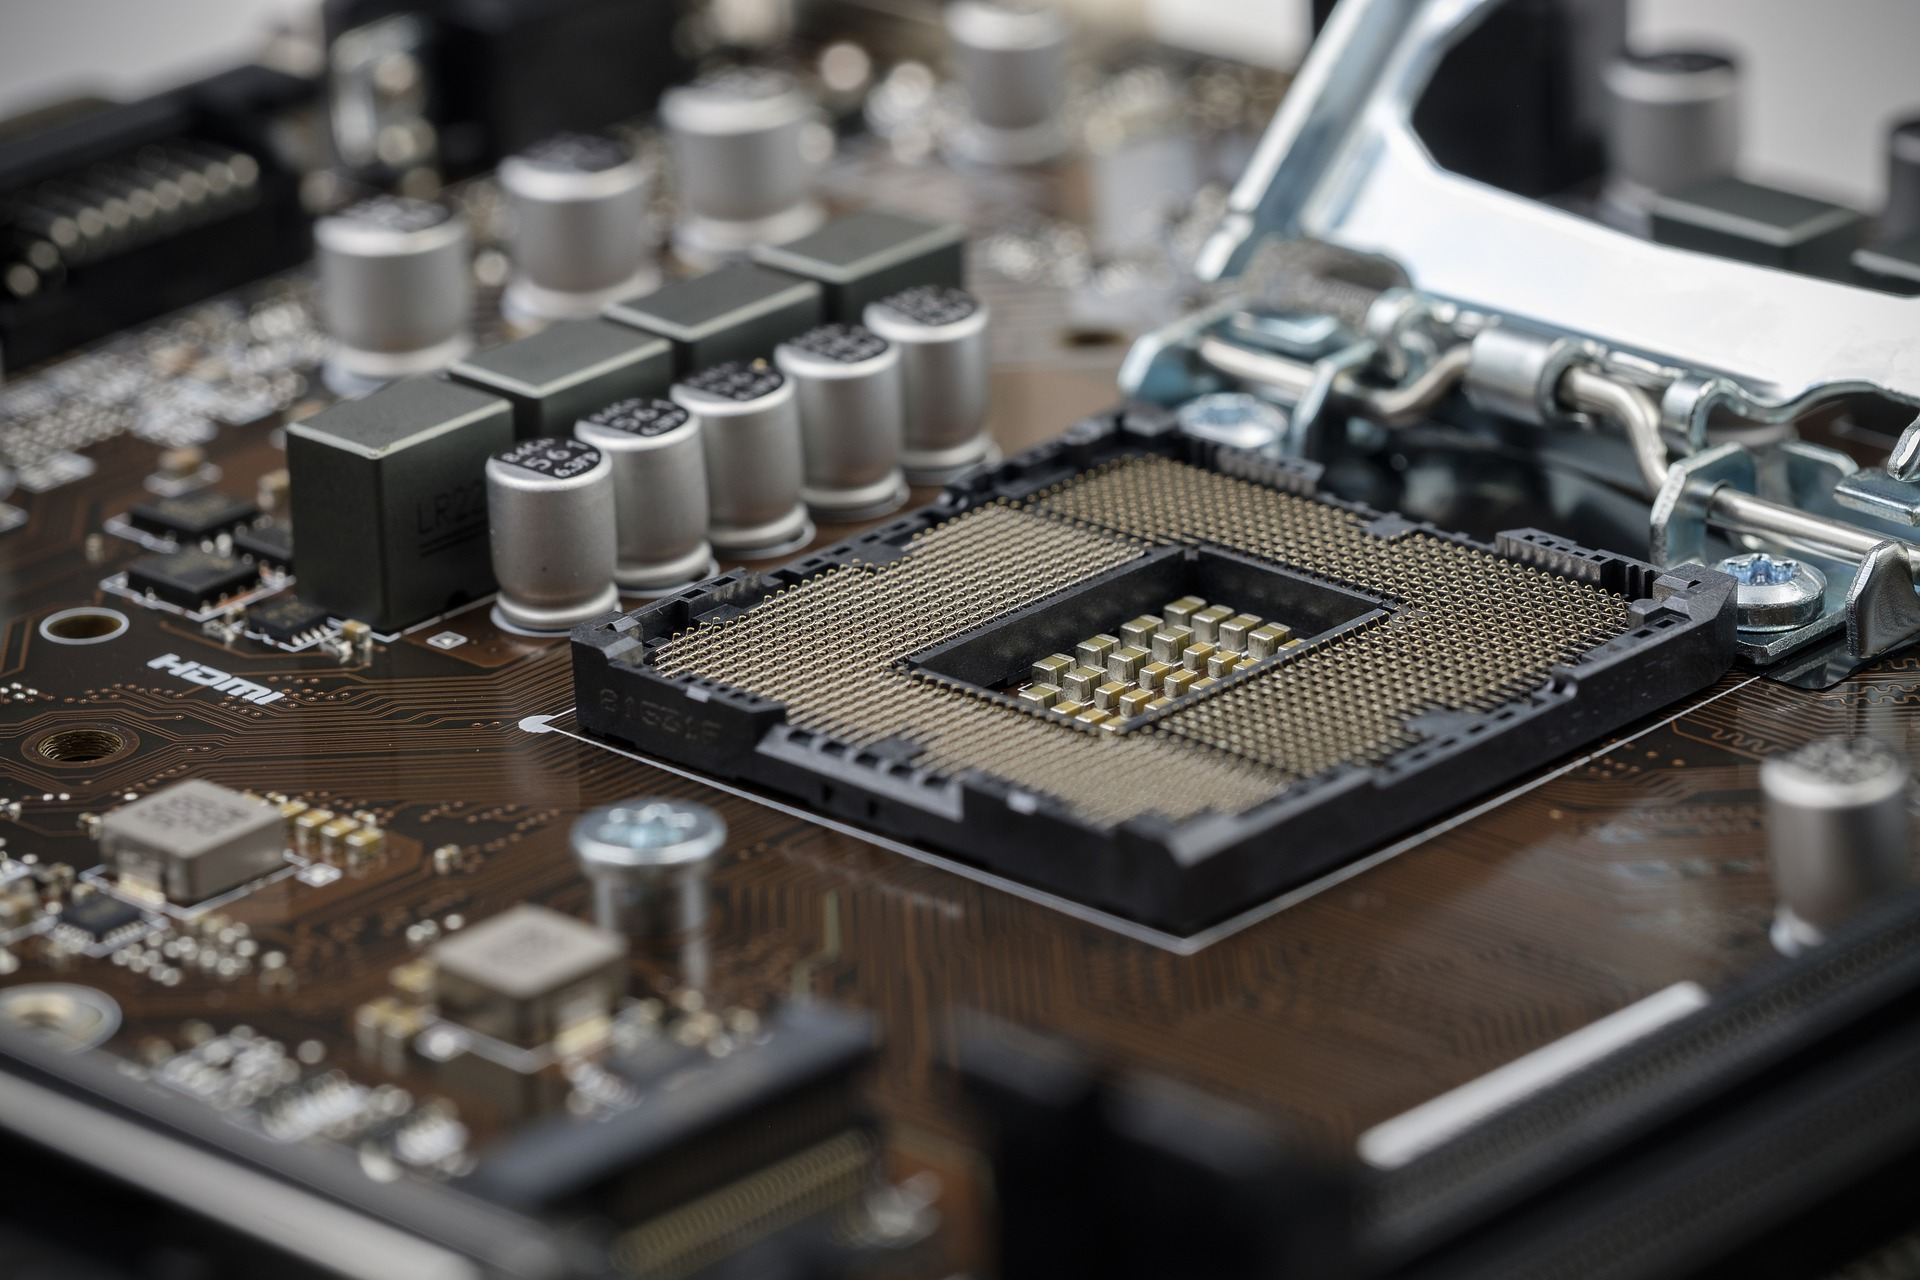
\includegraphics[width=0.3\paperwidth]{images/cpu-socket.jpg}
    \caption{Zócalo de CPU} \footnotesize
    Fuente: Imágen por \href{https://pixabay.com/users/bru-no-1161770}{Bruno /Germany} de \href{https://pixabay.com}{Pixabay} \cite{pixabay-cpu-socket-2019}.
\end{figure}

\section{Conclusión}

\printbibliography

\end{document}
